\subfloat[$p_{0\_int}(t)$]
{
	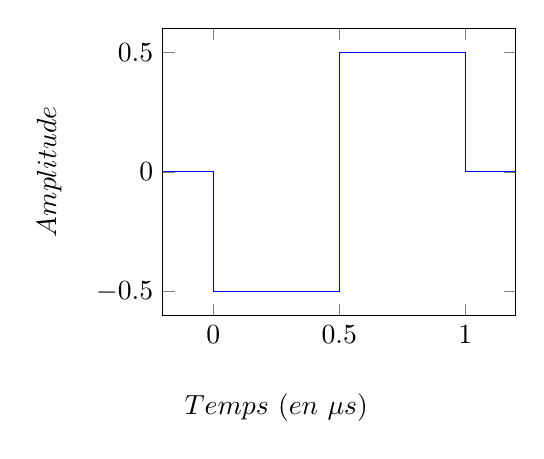
\begin{tikzpicture}
		\begin{axis}[
				xmin=-0.2,xmax=1.2,
				ymin=-0.6,ymax=0.6,
				xlabel={$Temps~(en~\mu s)$},
				ylabel={$Amplitude$},
				xlabel style={anchor=north, yshift=-0.4cm, xshift=-0.8cm},
				ylabel style={yshift=0.2cm},
				width=0.50\textwidth
			]
			\addplot[color=blue,mark=none] coordinates {
				(-0.2,0)
				(0, 0)
				(0, -0.5)
				(0.5, -0.5)
				(0.5, 0.5)
				(1, 0.5)
				(1, 0)
				(1.2, 0)
			};
		\end{axis}
	\end{tikzpicture}
}\hfill{}\subfloat[$p_{1\_int}(t)$]
{
	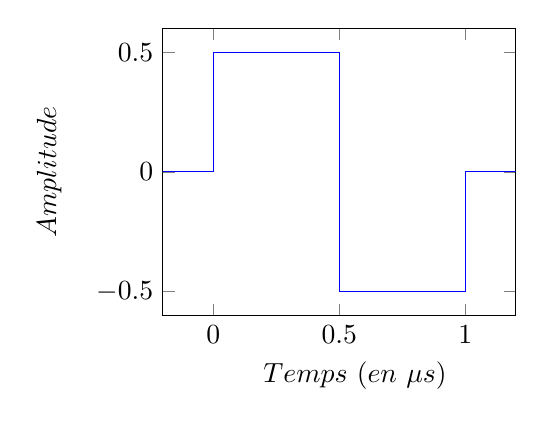
\begin{tikzpicture}
		\begin{axis}[
				xmin=-0.2,xmax=1.2,
				ymin=-0.6,ymax=0.6,
				xlabel={$Temps~(en~\mu s)$},
				ylabel={$Amplitude$},
				xlabel style={xshift=0.2cm},
				ylabel style={yshift=0.2cm},
				width=0.50\textwidth
			]
			\addplot[color=blue,mark=none] coordinates {
				(-0.2,0)
				(0, 0)
				(0, 0.5)
				(0.5, 0.5)
				(0.5, -0.5)
				(1, -0.5)
				(1, 0)
				(1.2, 0)
			};
		\end{axis}
	\end{tikzpicture}
}
